\section{视频系统}
乍看之下,视频输出系统 VGA(Video Graphic Array)仍是《德军总部 3D》所面对的那头怪兽:臭名昭著的 50 个寄存器、将颜色限制为 256 的调色板系统、以及尴尬的四个 64 KiB bank 迫使帧缓冲交错存储,都是令人不悦的编程接口。\\
\par
GC(Graphics Controller)与 SC(Sequencer)控制对 256 KiB 显存的访问。CRTC(Cathode Ray Tube Controller)控制帧缓冲的采样方式。最后由 DAC 将数字电平转换为模拟信号输出到 CRT。\\
\par 	
\scaleddrawing{0.6}{vga}{VGA 架构}
\par
在 90 年代初,大多数 PC 游戏使用 VGA 的“调制模式 13h”(也称 Mode-Y),分辨率为 320x200、每像素 1 字节、256 色调色板。使用这一未文档化模式,开发者直接操作显卡的四个 bank。帧缓冲在 bank 中的布局并不直观。如图 \ref{vga_ram_screen_layout} 所示,由于 RAM 访问速度历史上较慢,像素以 4 个为一组交错存储。




\cscaledimage{0.9}{vga_ram_screen_layout}{\label{vga_ram_screen_layout}}
\par
注意像素 \cw{0} 存在 bank 0,像素 \cw{1} 存在 bank 1,以此类推。水平分辨率为 320 列时,每个 bank 中存储 80 个在水平方向不相邻、但在垂直方向相邻的像素\footnote{VGA 设计是一个很大的话题,在 \it{Game Engine Black Book: Wolfenstein 3D} 中有详尽介绍。}。\\
\par
为访问 256 KiB 显存,IBM 在 RAM 中建立了一个硬编码映射,从 \cw{0xA0000} 到 \cw{0xAFFFF}。对十六进制习惯的人会立刻注意到:\cw{0xFFFF} 代表 64KiB 的地址空间,远小于可用显存容量。\\
\par
 为弥补地址不足,IBM 设计了通过 \textit{map mask register} 管理的 bank 切换系统。实际上,这意味着 RAM 中 \cw{0xA0000} 到 \cw{0xAFFFF} 的地址可以映射到显存中的四个位置,如图 \ref{ram_vram_mapping} 所示。掩码很繁琐,但带来了魔法,例如一次写入即可写四个像素\footnote{VGA 掩码技巧在 \it{Game Engine Black Book: Wolfenstein 3D} 中讨论。}。

% {
% \setlength{\belowcaptionskip}{-5pt}
\scaleddrawing{1}{vga_mapping}{\label{ram_vram_mapping}} \label{vga_ratio}
% }
\par
\vspace{-10pt}
另一个困难来自 mode Y 帧缓冲布局与 CRT 显示的纵横比不同,导致图像失真。 \\
\par
% {
% \setlength{\belowcaptionskip}{-5pt}
\cfullimage{circleframebuffer.png}{\label{circle_framebuffer}}
% }
\vspace{-10pt}
\par
图 \ref{circle_framebuffer} 中,程序员在帧缓冲里画了一个圆;注意 $ 320/200 = 1.6 $ 的纵横比。\\
\par
\cfullimage{circlescreen.png}{\label{circlescreen}}
\par
图 \ref{circlescreen} 展示了同一帧缓冲在显示器上呈现的样子。注意 $ 320/240 = 1.333 $ 的纵横比。圆因此变成椭圆。\\








\section{隐藏的改进}
尽管描述看似阴暗,但深入观察显卡世界会发现两项重大变化,最终深刻影响了 \doom。 \\
\par
自 1992 年起,微软与 IBM 发布新操作系统(Windows 3.1 与 OS/2 2.0)后,对高速显卡的需求迅速增长。对原本只需在文本模式下搬运 4,000 字节信息\footnote{2,000 字节用于字符,2,000 字节用于屏幕属性} 的设备而言,能驱动 GUI 的 153,600 字节\footnote{640x480,16 色} 是一场巨大技术飞跃。

\fullimage{Windows311workspace.png}\\
\par 
尽管界面简单,Windows 3.1 的 640x480、16 色就足以让 PC 累垮。移动窗口时必须只画轮廓,因为硬件刷新速度不够快,无法同时显示内容\footnote{\NeXT 工作站可以做到,Steve Jobs 经常在演示中提到 :)!}。



\subsection{VGA 芯片厂商}
第一项改进来自 VGA 芯片厂商。意识到性能需求的增长,ATI、Cirrus Logic 与 Tseng Labs 等公司投入巨大努力竞争并提升性能。硬件 GUI 加速尚未主流,因此图形应用的重绘速度主要受主机吞吐量影响。他们开始把 VGA 卡的所有组件紧密集成到一颗芯片中(RAM、RamDAC、BIOS、内存控制器、Blitter、内存刷新、缓存控制器、时序控制器\footnote{Tseng Labs ET4000} 等等)。\\
\par
有些厂商(如 Cirrus Logic)甚至采用无晶圆厂模式,出售半导体设计而将制造外包。


一个优化手段是利用 VGA RAM 写操作远多于读操作的特点。通过 FIFO SRAM 缓存来缓冲写入并立即返回,可显著提升屏幕 blit。以 Tseng Labs 那个年代最著名的芯片之一 ET4000 为例,可以一窥用户能买到的显卡。\\ 
\par
\cfullimage{vlb_cards/tseng_lans_et4000_w32_vesa_local_illetw32.png}{ILLETW32 Britek Electronics。图片来自 \cw{http://www.amoretro.de/}}
\par
通过授权 ET4000 \circled{1},Britek Electronics 只需提供 RAM \circled{2}、RAMDAC \circled{3}、计时器 \circled{4},并通过可编程阵列逻辑 TIBPAL16L8 \circled{5} 做少量定制。VGA BIOS 芯片 \circled{6} 也可从 Tseng Labs 购买。\\
\par
\vspace{10pt}
\drawing{vga_vlb_arch}{}

\par



\subsection{VL-Bus}
无论显卡厂商如何优化产品,仍有一处巨大瓶颈不受其控制:CPU 写入的信息必须经过 ISA 总线。\\
\par
ISA 总线在 1981 年推出,最初为 8 位数据通路,运行频率 4.77 MHz。1984 年升级到 16 位、6 MHz。服役 10 年后,它已显老态,被视为性能杀手。\\
\par
\drawing{bus_isa}{ISA 总线}
\par
对现状不满的硬件厂商联合成立 VESA(Video Electronics Standards Association),制定了新总线标准。他们并没有采用复杂协议,而是直接使用 Intel 486 Bus Unit 协议,使其几乎无摩擦地应用。\\
\par 
VLB(VESA Local Bus)将 ISA 的数据线翻倍为 32 位,并将频率提高到 33 MHz,比 16 位 ISA 快了可达 10 倍。\\
\par
VLB 控制器芯片设计相对简单,因为许多核心指令(中断与端口映射 I/O)仍由主板上的 ISA 电路处理,而内存映射 I/O 与 DMA 数据通路位于 CPU 同一条本地总线(见图 \ref{bus_vlb})。系统数据总线的速度基于主板晶振频率,这意味着总线与 CPU 同速运行。\\
\par
\drawing{bus_vlb}{VL-Bus,也称 VESA Local Bus,也称 VLB}
\label{vlbarchitecture}

\par
将 VL-Bus 架构紧密绑定到 486 Bus Unit 带来了无与伦比的性能,也使得采用非常容易,因为不需要芯片组。“本地总线”的含义是地址、数据与控制信号直接连接到处理器,因此设备只需通过电气缓冲即可连接。这是其简洁的原因之一,但也带来了许多限制。\\
\par
因为必须与 CPU 同速运行,当频率达到 40 MHz 时,VL-Bus 会变得不稳定并导致崩溃。超过这一速度后,系统对时序偏差越来越敏感\footnote{这一问题不影响 486 DX-66MHz,因为其总线仅 33MHz。}。根本原因在于“本地总线”按定义是同步的。扩展卡厂商必须确保其产品能在多种频率下运行,而上限会随着新处理器出现而提高。这注定导致兼容性问题\footnote{使用 AMD 80MHz、总线 40MHz 的 VL-Bus 系统就曾遭遇此类问题。}。\\
\par
第二个问题是,CPU 对总线施加的电气负载会随着时钟频率提升而下降。在 33MHz 下可提供 3 个插槽,但在 40MHz 下只剩 2 个,在 50MHz 时仅剩 1 个。这导致配置地狱,因为主板频率可调但仍提供三个插槽。用户会发现某些 VLB 插槽“无法使用”或“停止工作”。\\
\par
卡很难安装,因为卡体很长,需要用力插入 VLB 插槽,可能导致物理损坏\footnote{朋友们戏称 VLB 为 “Very Long Bus”。}。\\
\par
 最糟糕的是,Intel 在 1993 年推出的 Pentium Bus Unit 协议基于 PCI,完全不兼容。无法适配,VL-Bus 在一年内即告过时并消亡。\\
\par

\begin{figure}[H]
\centering
  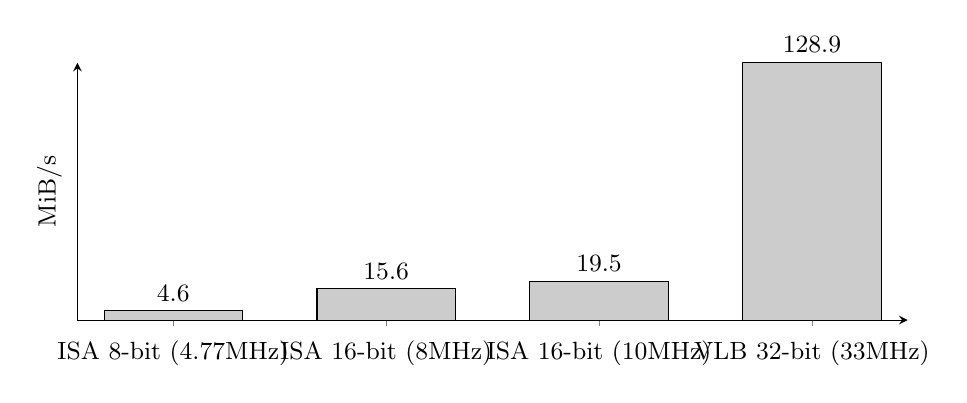
\begin{tikzpicture}[font=\small]
    \begin{axis}[
      width=1.0\textwidth,
      height=0.4\textwidth,
      ybar,
      bar width=50pt,
      ylabel={MiB/s},
      ymin=0,
      ytick=\empty,
      xtick=data,
      axis x line=bottom,
      axis y line=left,
      enlarge x limits=0.15,
      symbolic x coords={ISA 8-bit (4.77MHz), ISA 16-bit (8MHz),ISA 16-bit (10MHz), VLB 32-bit (33MHz)},
      xticklabel style={anchor=base,yshift=-\baselineskip},
      nodes near coords={\pgfmathprintnumber\pgfplotspointmeta}
    ]
      \addplot[fill=black!20,draw=black] coordinates {
        (ISA 8-bit (4.77MHz),4.6)
        (ISA 16-bit (8MHz),15.6)
        (ISA 16-bit (10MHz),19.5)
        (VLB 32-bit (33MHz), 128.9)
      };
    \end{axis}
   
   \end{tikzpicture}
   \caption{理论最大速度(MiB/sec)\protect\footnotemark。}
 \end{figure}
\par
\footnotetext{至少有一个周期用于在总线上放置地址,这会使有效带宽减半。}
% VL-Bus design specifications provides two other performance-boosting features: burst mode and bus mastering. In burst mode, VLB devices gain complete control of the external data bus for up to four bus cycles, passing up to 16 bytes of data in a single burst (which was conveniently exactly the size of a 486 cacheline). Bus mastering allows the VLB controller to arbitrate data transfers between the external data bus and up to three VLB devices without assistance from the CPU.\\
% \par
下一页展示了 1994 年可用的三张 VGA 卡。连接器一眼就能看出其总线类型与性能。\\
\begin{itemize}
\item 上:ATI 8800,ISA 8 位接口。
\item 中:ATI Mach32,ISA 16 位接口。
\item 下:Cirrus Logic MachSpeed,VLB 32 位接口。
\end{itemize}
注意 VLB 连接器仅使用 ISA 连接器的 8 位部分,但没有 16 位部分的齿口。
 
\scaledimage{0.93}{vlb_cards/ati8800.png}\\

\vspace{5mm}

\scaledimage{0.93}{vlb_cards/ati_mach32.png}\\

\vspace{5mm}

\scaledimage{0.93}{vlb_cards/Cirrus_Logic_CL-GD5429.png}
